\chapter{Introduction}\label{chap:intro}

\begin{quotation}
\noindent 
In this chapter we introduce some of the motivating factors and the context of the research work presented in this thesis. We outline the three research questions this thesis is centered around and we describe the methods used to address them. We also present the related work and state the high-level contributions of the thesis.

This chapter is based on the paper entitled \textit{User-generated metadata in audio-visual collections} which was presented at the Doctoral Symposium of the 21st International World Wide Web Conference (WWW2012), held in Lyon, France.
\end{quotation}

\section{Context and Research Problems}
The central goal of this research work is to investigate the added value of user-generated metadata in professionals environments such as audio-visual archives. 
\subsection{Audio-visual Collections in the Digital Era}
Audio-visual (AV) content collections are undergoing a transformation from archives of analogue materials to very large stores of digital data accessible online. Prerequisite for successful information retrieval and collection management is quality metadata associated with collection items. Traditionally, the task of annotating video programs is strictly in the hands of professional cataloguers who adhere to well-established guidelines in the cataloguing process \cite{acrchivingphilosophy}. Usually, the resulting manually-crafted professional annotations are coarse-grained in a sense that they are referring to the entire program describing the prevalent topics. Fine-grained manual annotation of video fragments, on the other hand, is prohibitive, as the work involved is inevitably tedious, incomplete, and costly \cite{bouke}. However, a significant portion of user-content requests are targeted at video fragments rather than entire programs; a transaction-log analysis \cite{fragmentpercent} performed in a broadcast archive showed that fragment purchases account for 66\% of all purchases. As the program level professional annotations may be inadequate for locating or retrieving of fragments --- or any other task that involves fragments rather than entire programs --- the need for fine-grained annotations becomes clear. A possible solution to the problem of scarcity of fine-grained
 video metadata is to harness users' efforts to amass video fragment-level descriptions.
 
One of the most common forms of user-generated metadata are \textit{tags}. With the advent of the Web 2.0 the tagging phenomenon witnessed rapid proliferation in many
areas; image collections\footnote{http://www.flickr.com}, bookmark collections\footnote{http://www.delicious.com}, user video collections\footnote{http://www.youtube.com}. Experience has shown that joint efforts of user communities result in massive amounts of tags usually unparalleled --- in terms of quantity --- by what professionals can provide. Just to put things into perspective, in 200 years of existance the Library of Congress has applied their expert-maintained taxonomy to 20 million books\footnote{http://www.loc.gov/about/reports}, whereas, in only four years, Flickr's users applied their ad-hoc tagging vocabulary to over 25 million photos. This suggests that there is, indeed, a potential in engaging end-users in the video-annotation process. One way of achieving this is through so-called `games with a purpose' \cite{gwap}. To this end, the Netherlands Institute for Sound and Vision\footnote{http://portal.beeldengeluid.nl/} (S\&V) in cooperation with KRO broadcasting\footnote{http://www.kro.nl/} launched \textit{Waisda?} in May 2009, a multi-player video labeling game where players describe streaming video by entering tags and score points based on temporal tag agreements . The underlying assumption is that tags are probably valid --- trustworthily describe the video fragments --- if they are entered independently by at least two players within a given timeframe (see figure \ref{fig:waisda}). The motivation behind \textit{Waisda?} is to improve the access to S\&V collection~\cite{johanwebsci}. With \textit{Waisda?} the S\&V institute aims to collect metadata in a user vocabulary, as previous research \cite{Jorgensen2007} suggests that such metadata can help bridge the gap between the search queries and the indexing vocabulary. In addition, it is expected that the resulting time-related metadata of the content within the video can improve support for finding fragments within entire broadcasts~\cite{bouke}.

\begin{footnotesize}
\begin{figure}[t!]
\centering
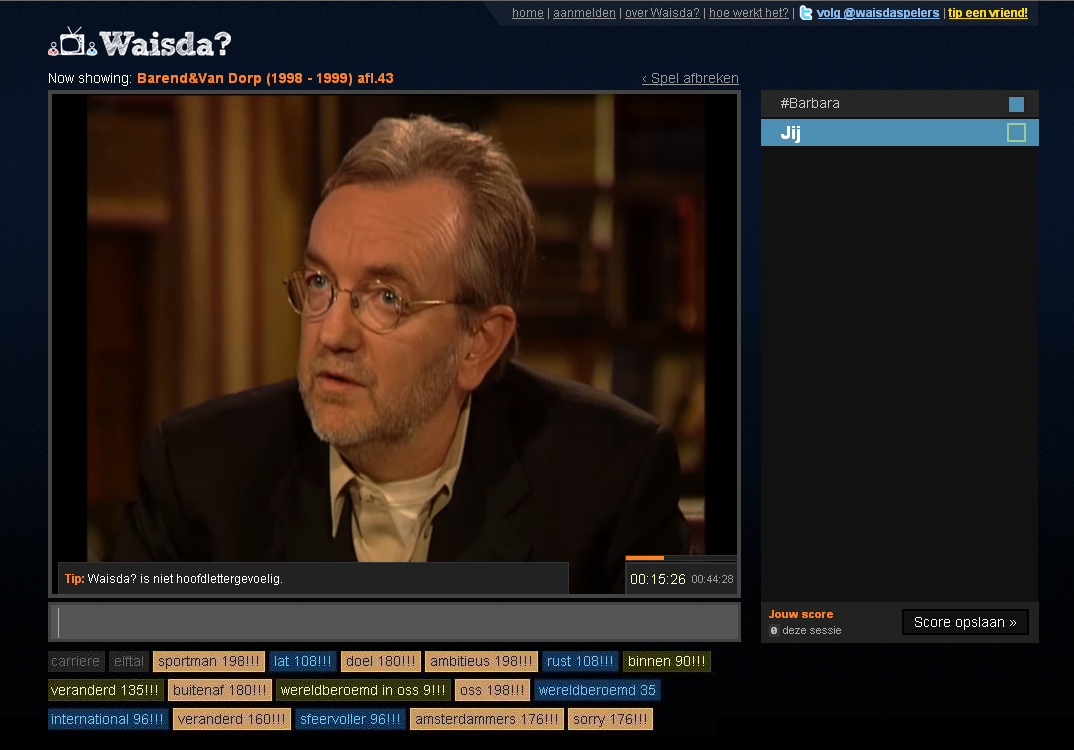
\includegraphics[scale=0.5]{intro:waisda_game}
\caption{Screenshot of the \textit{Waisda?} game interface: the central part of the screen is reserved for the video. Immediately below the tag input field and the list of tags entered already are placed. The coloration of the tags is indication of the number of points the tags scored.  On the right, there is the list of players currently in the game.}
\label{fig:waisda}
\end{figure}
\end{footnotesize}

\subsection{Project context}
This research is part of and funded by the \textit{PrestoPRIME}\footnote{http://www.prestoprime.org/} project which brings together various European audiovisual archives (including S\&V), research institutions, and industry partners. PrestoPRIME develops practical solutions for the long-term preservation of video and audio broadcasts, and finds ways to increase access by integrating the media archives with European on-line digital libraries. One of the considered ways to increase accessibility to videos is by exploiting user-generated tags collected through the labeling game \textit{Waisda?}.

\subsection{Research questions}\label{sec:research-questions}
The overall problem statement for this research is as follows.
\begin{quote}
\textit{What potential added value do user-generated video annotations have in professional environment?}
\end{quote}

To successfully integrate user-generated tags into AV collections' workflows a better understanding of their characteristics, compared to preexisting professionals annotations, is required. In particular,  the terminology that users employ when describing videos  and the aspects of the video that they usually describe. The first research question, therefore, is
\begin{itemize}
	\item[1.] What are the relationships between user-generated tags  and professional annotations in terms of the vocabulary and what they describe?
\end{itemize}
Locating a fragment within a video is an important use case in AV collections for which the fine-grained user tags could potentially provide an added value. Thus, the second research question addresses the usefulness aspect of user tags in terms of locating fragments within a video.
\begin{itemize}
	\item[2.] Can we improve fragment search  within video, with the help of user-generated data?
\end{itemize}
%Previous research \cite{websciencepaper,kcap,johanwebsci} has shown that user tags predominately describe objects and rarely refer to topics of a scene. Considering that professional annotations at scene-level are scarce, we investigate whether user tags can be used to deduce what the scene is about. Therefore, the third research question is
%\begin{itemize}
%	\item[3.] Can we derive topical description for scenes from user-generated tags?
%\end{itemize}

Lastly, successful integrations of user tags also requires that issues around assessing and improving tag quality to be addressed. The third and final research question, therefore, is
\begin{itemize}
	\item[3.] Can the quality of user-generated tags for videos be evaluated and improved?
\end{itemize}

\section{Related Work}
In this section we outline some of the related work. It should be noted that this is an incomplete list of the more relevant studies.
\subsection{Games With a Purpose}
Games with a purpose (or GWAPs) are computer games, in which people, as a side effect of playing, perform tasks computers are unable to perform \cite{gwap}. The first example of a GWAP was the ESP game \cite{CHI2004:vonAhn}, designed by Luis von Ahn, which harnesses human abilities to label images. %The game randomly pairs up two players with the task to describe images. When both players provide the same label for an image, they score points and proceed to the next image. The labels entered by both users are associated to the image as metadata. In other words, the consensus among users provides a method to ensure the quality and consistency of the labels. Evaluation shows that these labels can be used to retrieve images with high precision and are almost all considered as good descriptions in a manual assessment.
The idea to collect metadata through games with a purpose has been applied to video footage in, for example, the Yahoo! video tag game \cite{WWW08_vanZwol_etal},
VideoTag\footnote{http://www.videotag.co.uk/}, PopVideo\footnote{http://www.gwap.com/gwap/gamesPreview/popvideo/} and \textit{Waisda?}. Compared to the other video labeling games, \textit{Waisda?} is unique in the sense that it is initiated by an audiovisual institute (S\&V) with the purpose to improve the access to their collection~\cite{johanwebsci}.

\subsection{Evaluation of End-user Tags in Professional Environment}
The Steve project \cite{MATW2009:Leason} was one of first attempts to explore the role of user-generated metadata. In this collaboration of several art museums a collection of artworks was made available to the general public who were asked to tag them. Among other things, the project studied the relationship of the resulting folksonomy to professionally created museum documentation. The results showed that users tag the artworks of art from a perspective different than that of museum documentation: around 86\% of tags were not found in museum documentation.

Museum staff also assessed the tags from the steve.museum project on usefulness when used to search for artworks. From the total number of tags, 88.2\% were found to be useful. Following the methodology of steve-museum, S\&V institute also asked a senior cataloguer to judged a sample of \textit{Waisda?} tags on their usefulness when searching for videos \cite{johanwebsci}. The sample consisted of the 20 most frequent and the 20 least frequent tags from two television programs. The cataloguer found the majority of the tags to be useful. She also noted that there seems to exist a difference between professional descriptions and end-user tags. While professionals describe the topical subject of the program, the players in \textit{Waisda?} generally tag things that can be directly seen or heard in the video. One of the aims of this research is to investigate the characteristics of the tags and what they describe in the video more methodically, and on a larger scale.

\subsection{User annotations for search}
Search based on user-generated metadata, in particular folksonomies, has been studied before. Morrison compared web search performance of folksonomies from social bookmarking web sites against search engines and subject directories \cite{morison}, showing that search engines had the highest precision and recall rates. Folksonomies, however, performed surprisingly well. In fact, user tags show promise to alleviate the vocabulary mismatch problem for search: bridging the gap between user queries and metadata used for retrieval \cite{vocprob}. Indeed, Geisler and Burns state that YouTube tags provide added value for search, because 66\% of them do not appear in  other metadata \cite{youtube}. Heymann et al. investigated a large-scale sample of forty million bookmarks from the social bookmarking site del.icio.us and found that in 20\% of the cases user tags do not occur in the page text, backlink page text, or forward link page text of the pages they annotate. Studies in \cite{Bischoff:2010:BGT:1833903.1834001,Halvey:2007:AOV:1286240.1286301,journals/jasis/Rorissa10,Yanbe:2007:SBE:1255175.1255198} investigate this phenomenon across multiple domains and multimedia resource types and identify the gaps between the tag space and the querying vocabulary. The common conclusion is that user tags can improve search by bridging the vocabulary gap. 

Studies reported in \cite{Bischoff:2008:TUS:1458082.1458112,Sun:2010:QTR:1873951.1874029} take a more critical stance. They conclude that while overall user tags improve search, not all tags are suitable for retrieval. This hints that a characterization of the quality of the tags is needed to filter out the tags that are not suited for retrieval. This is one of the aspects that we address in this thesis. 

Another line of research is exploiting the tripartite structure ($Users \times Tags \times Resources$) of folksonomies to improve search \cite{Hotho:2006:IRF:2094613.2094652,Bao:2007:OWS:1242572.1242640}. Alternatively, the semantics of tags can be grounded in some lexical sources and the grounded tags utilized for improving search. For example, Hildebrand et al. proposed and investigated a semi-automatic process of assigning explicit meaning to user tags for video by linking them to concepts from the Linked Open Data cloud \cite{michiel}.

\subsection{Quality and Refinement of Annotations}
There is a substantial body of research into the refinement and quality assessment of annotations of still images. Lee at al. propose a tag refinement technique that aims at
differentiating noisy tag assignments from correct tag assignments \cite{Lee:2010:TRI:1890924.1891010}. Each tag is assigned a probability of being noisy based on the visual similarity of the images and tag co-occurrence statistics. Tags with a probability below a threshold are discarded as noisy. 

In \cite{Truong:2012:CSK:2324796.2324808,Li:2008:LTR:1460096.1460126} neighbour voting schemes for determining the tag relevance are explored. In this approach, a tag is considered more relevant to the image it is ascribed to, also known as the seed image, if the tag is also used to annotate the neighbouring images. The neighbourhood relation is defined in terms of the visual similarity among images. Lee at al. expand the approach by not only considering the visually similar images, but the dissimilar images as well, thus providing negative examples \cite{Lee:2012:TDE:2390876.2390880}. Kennedy at al. exploits visual similarity among images in a sense that tags ascribed to images by the creators of the image are used as seed annotations and also attached to visually similar images \cite{Kennedy:2009:RTU:1631135.1631139}. Zhao at al. propose a data-driven method to automatically determine the relatedness between a tag and the image's visual content taking into consideration the tag co-occurrence and the visual similarity among images \cite{Zhao:2010:TRV:2174490.2174571}.

Probabilistic methods that exploit random walk based techniques have also been explored \cite{Wang:2006:IAR:1180639.1180774,Liu:2009:TR:1526709.1526757,Li:2012:TRP:2382336.2382380}. These methods produce a ranking of the tags according to their relevance with respect to the image with which they are associated. The tag relevance estimations are computed as the stationary or the convergence probabilities of  a random walk processes. Notable example of this approach is the PageRank algorithm \cite{journals/corr/abs-1012-4872,10.4137/GRSB.S702,junker2008analysis}. Another group of methods exploit background knowledge (such as the lexical database Wordnet and a massive corpus indexed by Google) to perform the refinement of the image annotations \cite{Jin:2010:KBI:1731523.1731529,Wang:2007:RIA:1282280.1282343}. The semantic relations encoded in Wordnet and the semantic similarity quantified by the Google-based measures like the Normalized Google Distance \cite{DBLP:journals/corr/abs-cs-0412098} provide contextual evidence for the relationship among the annotations. This evidence is then used as an input for machine learning algorithms which give the final word for the quality of the annotations.

\section{Approach}
In this section we outline the approach to answer the research questions stated above. The specific approach for each of the research questions is described in separate subsection. The order of the subsections is respective to the order in which the research questions are stated in section \ref{sec:research-questions}. At the basis of each of the approaches lies \textit{Waisda?} which was used as a data-collection tool. In the course of this thesis significant effort went into improving the game design and development of software extension that enables seamless integration of the game into larger workflows. Chapter \ref{chap:waisda} describes the game in more detail and outlines the contributions of this thesis with respect to the development of the game.

\subsection{\textit{Waisda?} User Tags vs. Professional Annotations}\label{sec:user-professional}
To answer the first research question `What are the relationships between user-generated tags  and professional annotations in terms of the vocabulary and what they describe?' we perform two studies. Details can be found in \cite{websciencepaper,kcap}.

The first study is a quantitative data analysis of the entire tag collection gathered with \textit{Waisda?} during the first six months after the game was deployed. In order to estimate the lower bound of the fraction of user tags that are meaningful words, we examine the overlap between them and general lexical resources and vocabularies. Furthermore, to determine if users and professionals use different vocabularies when describing videos, we investigate the overlap between all user tags and a typical domain thesaurus used by professionals in the cataloging process. The results from the study show that there is, indeed, a terminological gap between users and professionals; while approximately 89\% of all user tags are meaningful words only 8\% of them were found in the domain thesaurus used by professionals.

In the second study, we take a combined approach. First, we investigate what do users tend to describe  more: things \textit{heard} or things \textit{seen} on screen. To this end, we perform a study on the overlap between the user tags and the audio signal --- subtitles for hearing impaired persons --- for a sample of episodes. Second, to get a more comprehensive understanding of the types of tags users usually add, we perform a qualitative study of a sample of user tags obtained through the \textit{Waisda?} video tagging game. In particular, each tag from the sample is manually analyzed in the light of the video content it describes and categorized in terms of the Panofsky-Shatford classification framework. The results of the study show that user tags predominately describe objects and rarely refer to topics of a scene. This is in sharp contrast with the professional annotations which  exclusively target the topic(s) of the entire video and (lot less frequently) of particular scenes. 


\subsection{Investigating the Added-value of User Tags for Fragment Search}\label{sec:fragment-search}
Fragment search within video is widely recognized as an application scenario of particular business importance in the AV collections world \cite{fragmentpercent}. However, the existing professional annotations generally refer to the entire video and are not tied to a specific time-point, which decreases their usefulness for fragment retrieval; without temporal data one needs to manually locate the fragment of interest. \textit{Waisda?} tags, on the other hand, do refer to fragments and are time-based, with time codes that \textit{deep link} to particular point in the video. Our aim is to investigate their added-value for fragment retrieval. Furthermore, we plan to explore what kind of query tasks (search for \textit{events}, \textit{objects}, etc.)  benefit from the user tags.

The methodology that we consider is \textit{quantitative system evaluation} \cite{vorhees}. In order to evaluate effectiveness of information retrieval, this methodology requires collection of ``documents'' (in our case video fragments), set of queries, and relevance judgments  indicating which ``documents'' in the collection should be returned for each query. We plan to create evaluation dataset from the videos that were part of \textit{Waisda?} game deployment and tagged by players. For such a dataset real-life, authentic user tags would already be available. However, set of fragments, relevance judgements, set of queries and query task types need to be defined. The method of achieving this is going to be part of and one of the contributions of the research.
	
An alternative is to creating an evaluation dataset is using an existing one. There are various video retrieval evaluation initiatives like TRECVID\footnote{http://trecvid.nist.gov/} that provide datasets for testing content-based retrieval techniques. The advantages of reusing such a dataset are (i) the set of fragments is defined, (ii) the set of queries and the relevance judgments are defined. The drawbacks are that \textit{Waisda?} like games have not been run yet on this dataset and setting up such a game and attracting sufficient users for this material could turn out to be hard. Also we are limited to the query task types defined by the dataset. Our position is that the effort required to collect user tags for the material outweighs the advantages offered by this approach.
	


%\subsection{Deriving Topical Descriptions From User Tags}\label{sec:topical-desc}
%Video fragments or scenes are often multivalent in terms of their meaning and as such can be observed as a mixture of topics. User tags collected through \textit{Waisda?}, which are mostly referring to objects, can be seen as instantiations of these topics. The challenge that we are facing is to derive topical descriptions from the user tags. The unstructured nature of the tags, --- only weak temporal ordering of tags within video exists, based on the tag entry time --- makes statistical approaches excellent candidates  for this task. The research we have done so far puts statistical \textit{topic models} at the top of the list. Topic models \cite{Hofmann, Blei} are a type of statistical models for discovering abstract `topics' in collection of documents. One of the most common topic models currently in use is the  Latent Dirichlet Allocationc (LDA). The idea behind LDA is to model documents as arising from multiple topics, where a topic is defined to be a distribution over a fixed vocabulary of terms. Specifically, it is assumed that $\mathit{K}$ topics are associated with a collection, and that each document exhibits these topics with different proportions. Furthermore, LDA assumes that words are exchangeable within each document, i.e., their order does not affect their probability under the model. In other words, each document is treated as a `bag of words'. We believe that the assumptions underlying the LDA model are valid in and applicable to our context as well. \textit{Videos} and \textit{scenes within videos}, much like documents, have many layers of meaning and can be viewed as mixture of topics. The high-level professional \textit{topical} descriptions, on the other hand, can be considered as the analog to topics in LDA. The low-level user tags are referring to things heard or seen on screen and as such can be viewed as instantiations of the particular topics the video/scene is about. The unstructured and unordered nature of user tags --- in the borders of a particular shot/scene --- fits the 'bag of words' metaphor quite well. Regardless of the choice of the method the procedure we envision will proceed in four steps.

%\begin{enumerate}
%	\item \textit{Video segmentation}. Videos are segmented into shots (possibly scenes) using state of the art video analysis tools.
%	\item \textit{Tag-to-Shot association}. Tags are associated to the shots (scenes) derived in the first step. In this process the temporal information associated to each tag will be used and special attention will be payed to user tags assigned close to the detected boundaries.
%	\item \textit{Model training}. Statistical model is trained. The collection of topics used by the professional catalogers from the Sound and Vision Institute will be used as a list of abstract topics. We consider this set to be a representable and relevant for two reasons. (1) The videos that will be considered will originate from their catalogue. (2) Every single topical description in their catalog comes from this set. As a training corpus we shall use the Sound and Vision cataloque: each cataloque entry is annotated with topical descriptors and is associated to contextual documents that contain textual description of the program's content. Additional corpora may be used as well.
%	\item \textit{Topics inference}. Using the trained model, for each shot (scene), the most probable  topics will be inferred from the tags associated to it.
%\end{enumerate}

%We plan to evaluate the effect that the inferred topical descriptions will have on fragment retrieval. For this we will use the test data set from the fragment retrieval study described in section \ref{sec:fragment-search}.

\subsection{User Tag Quality Metrics}\label{sec:quality}
Our supposition is that any characterization of quality of the user tags is largely determined by how different institutions will use them. In other words, it is immaterial to talk about tag quality without a specific application scenario in mind. Fragment search within video is widely recognized as an application scenario of particular business importance in the AV collections world. For these reasons, our characterization(s) of tag quality will be limited to this scenario.  Some of the aspects we plan to investigate in the context of the retrieval scenario are tag frequency and discriminative power of tags,  correlation between reputation of players and tag relevance,  semantic ambiguity of tags, overlap with transcripts,  etc. The exact specifics of this study will be determined by the outcome of the previous studies. Therefore, we plan to make the choice of research methodology and the type of output (e.g. quantitative metrics or set of recommendations) this study will provide after the fragment retrieval study is performed.

\section{Structure of the Thesis}
The thesis is organized as follows. In Chapter 2 we study the characteristics of the tags collected with \textit{Waisda?}. In particular, we focus on two aspects. First, what is the relationship between the game  tags and the annotations created by professional catalogers. Second, we investigate which facets of the video content are typically targeted by the game tags and at what level of semantic specificity. In the following two chapters we study the effectiveness of game tags for video retrieval by addressing two prominent search scenario that arise in practice. In Chapter 3 we look into the first scenario which is retrieving videos that feature visual appearances of given objects of interest. In Chapter 4 we focus on the second scenario which is topical search, retrieval of videos that are about a given topic. In Chapter 5 we outline the technical specifications of \textit{Waisda?} and address two important points. First, how can \textit{Waisda?} be deployed and used by audio-visual collection owners to tag their collection. Second, how can \textit{Waisda?} be integrated into larger systems and workflows. Lastly, in Chapter 6 we present the overall conclusions of this thesis. We discuss the implications of this work and suggest directions for future research. 

\section{Publications}
Publications on which the chapters of this thesis are based:
\begin{itemize}
	\item Chapter 1 was published as: Riste Gligorov. User-generated metadata in audio-visual collections. In the \textit{Proceedings of the 21st international conference companion on World Wide Web (WWW 2012), Lyon, France, 2012.}
	\item Chapter 2 was published as: Riste Gligorov, Michiel Hildebrand, Jacco van Ossenbruggen, Guus Schreiber, and Lora Aroyo. On the role of user-generated metadata in audio visual collections. In the \textit{Proceedings of the International Conference on Knowledge Capture (K-CAP 2011)}, pages 145-151. ACM Press, June 2011.
	\item Chapter 3 was published as: Riste Gligorov, Michiel Hildebrand, Jacco Van Ossenbruggen, Lora Aroyo, and Guus Schreiber. An Evaluation of Labelling-Game Data for Video Retrieval. In \textit{Advances in Information Retrieval: 35th European Conference on IR Research (ECIR 2013)}, pages 50-61, Springer, Moscow, Russia, March 2013.
	\item Chapter 4 is an extension of: Riste Gligorov, Michiel Hildebrand, Jacco Van Ossenbruggen, Lora Aroyo, and Guus Schreiber. Topical Video Search: Analysing Video Concept Annotation through Crowdsourcing Games. In the \textit{International Journal of Human Computation 4(1)}, 47-66, 2017.
	\item Chapter 5 is an extension of: Michiel Hildebrand, Maarten Brinkerink, Riste Gligorov, Martijn Van Steenbergen, Johan Huijkman, and Johan Oomen. \textit{Waisda?}: video labeling game. In the \textit{Proceedings of the 21st ACM international conference on Multimedia}, pages 823-826, Barcelona, Spain, 2013. This publication describes the technical aspects of the game and the main author is Michiel Hildebrand. Chapter 5 incorporates the content of the publication and additionally, describes the contribution of the work carried out for this thesis on design and implementation of the game. 
	
\end{itemize}

\section{Contributions}
The main contributions of the thesis are:
\begin{itemize}
\item A method to analyze quantitatively the overlap between user and professional terminology exploited in video annotation.
\item Qualitative analysis of the aspects of the video content which are described by the game tags i.e. \textit{what do game tags describe in a video and how}.
\item A method to design a dataset ---including fragments, queries, and relevance judgements --- for evaluating the added value of user tags for \textit{visual} and \textit{topical} video search.
\item Two evaluation datasets ---one for visual and one for topical search --- which contain fragments, user tags from \textit{Waisda?} collection, queries, and relevance judgements.
\item Quantitative evaluation of the added value of the game tags in terms of \textit{visual} and \textit{topical} video search.

\item A method for qualitative analysis/classification of the search results in the context of visual search. The aim of the analysis was to discover the types of tags that are generally responsible for false positives.

\item Qualitative analysis of the search results in the context of topical search. The aim of the analysis was to discover tagging practices that generally produce relevant topical tags.

\item Evaluation of tag-related measures for accessing the quality of the game tags as topical descriptors in the context of topical video search.

\item Development of extension module for \textit{Waisda?} which enables integration of the game in AV collection workflows. The module is part of the latest release of \textit{Waisda?} which is available online\footnote{The \textit{Waisda?} source code and documentation is available from Github \url{http://github.com/beeldengeluid/waisda}}.
\end{itemize}

